\section{Architecture}
\label{sec:architecture}

% Overview of SRAM blocks
The OpenRAM SRAM architecture is based on a bank of memory cells
with peripheral circuits and control logic as illustrated in
Figure~\ref{fig:structure}. These are further refined into eight major
blocks: the bit-cell array, the address decoder, the word-line drivers,
the column multiplexer, the pre-charge circuitry, the sense amplifier,
the write drivers, and the control logic.

\begin{figure}[tb]
\centering
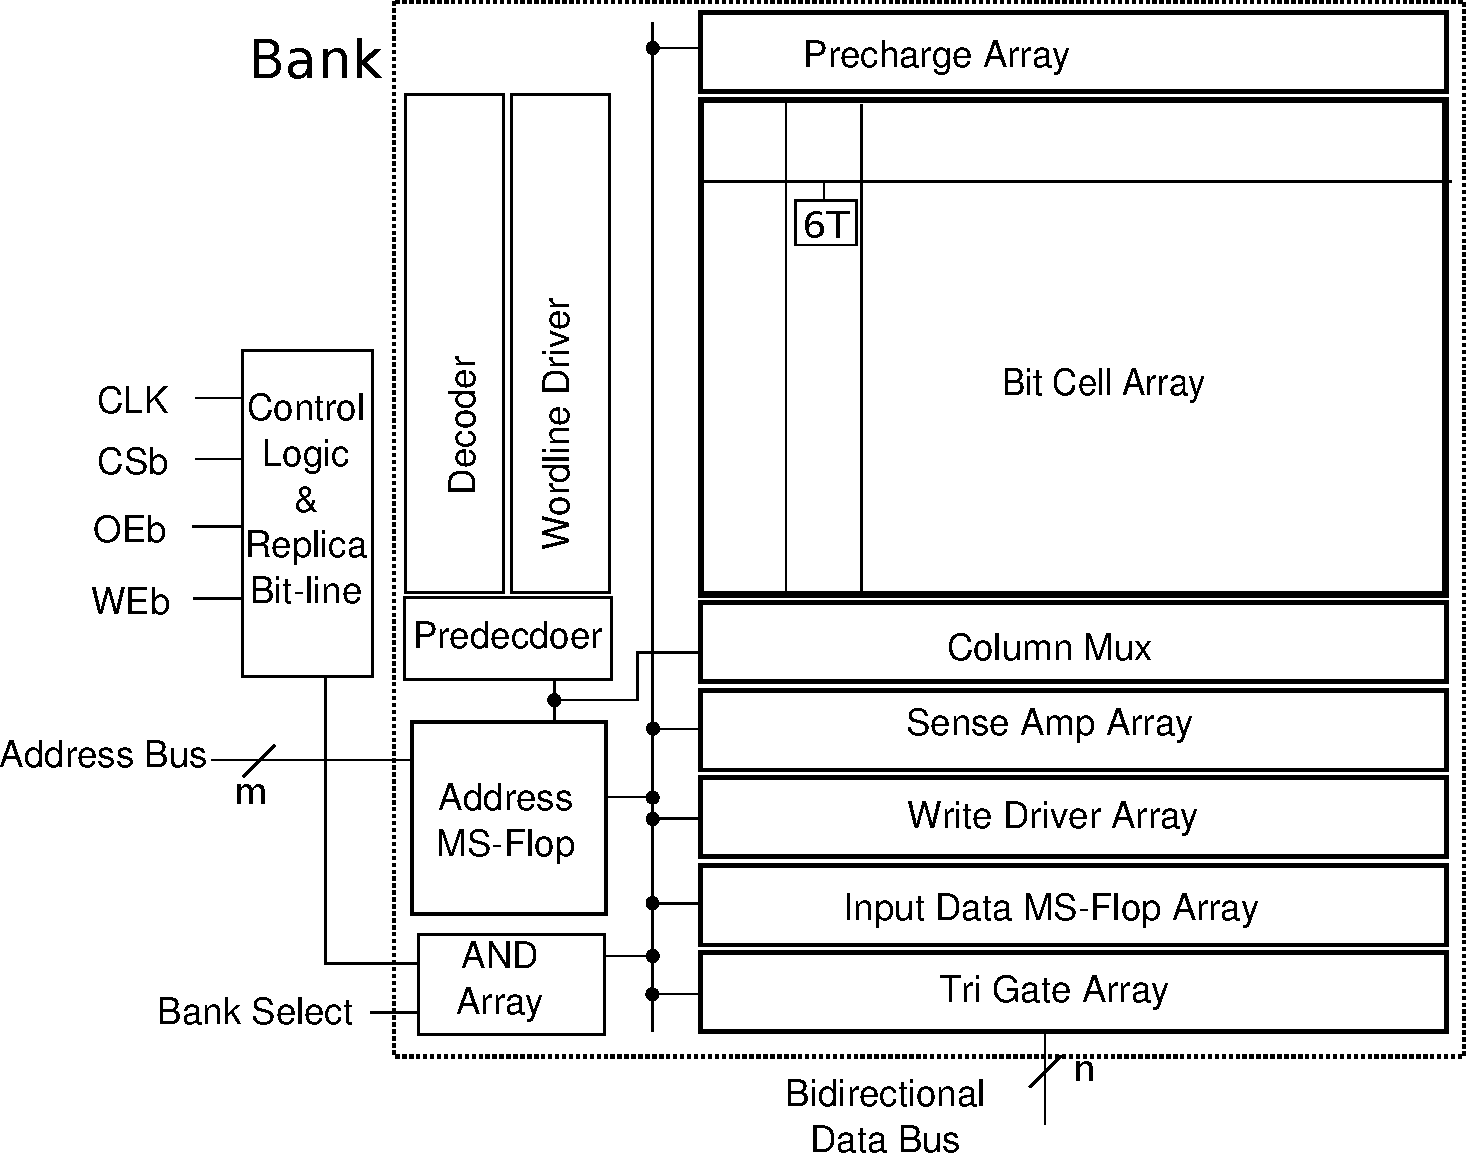
\includegraphics[width=8cm]{./figs/sram_structure.pdf}
\caption{An OpenRAM SRAM consists of a bit-cell array along with decoder, 
  reading and writing circuitry and control logic timed with a replica
  bit-line.
\label{fig:structure}}
\end{figure}

% we don't implement these yet, so don't give a tutorial on them
%% General memories and Register Files (RF) are both examples of what an
%% memory compiler can generate. General memories usually have shared
%% read/write ports whereas RFs typically have separate ports. All of
%% these options are permitted through the use of different types of
%% memory cells such as 6, 8, and 12 transistor (T) cells which contains
%% 1-4 access transistor pairs and their associated bit-lines. Some basic
%% memory array options are available below:
%% \begin{itemize}
%% \setlength{\itemsep}{0pt} \setlength{\parskip}{0pt}
%% \item Standard 6T cell for single-port memory
%% \item Dual-port 8T cell for dual-port memory or separate read/write ports
%% \item Four-port 12T cell for dual separate read/write ports
%% \item Custom sense amplifier designs for different performances
%% \item Different types of address decoders for different performances
%% \end{itemize}

\begin{figure*}[tb]
\centering
\subfigure[Read operation timing]{
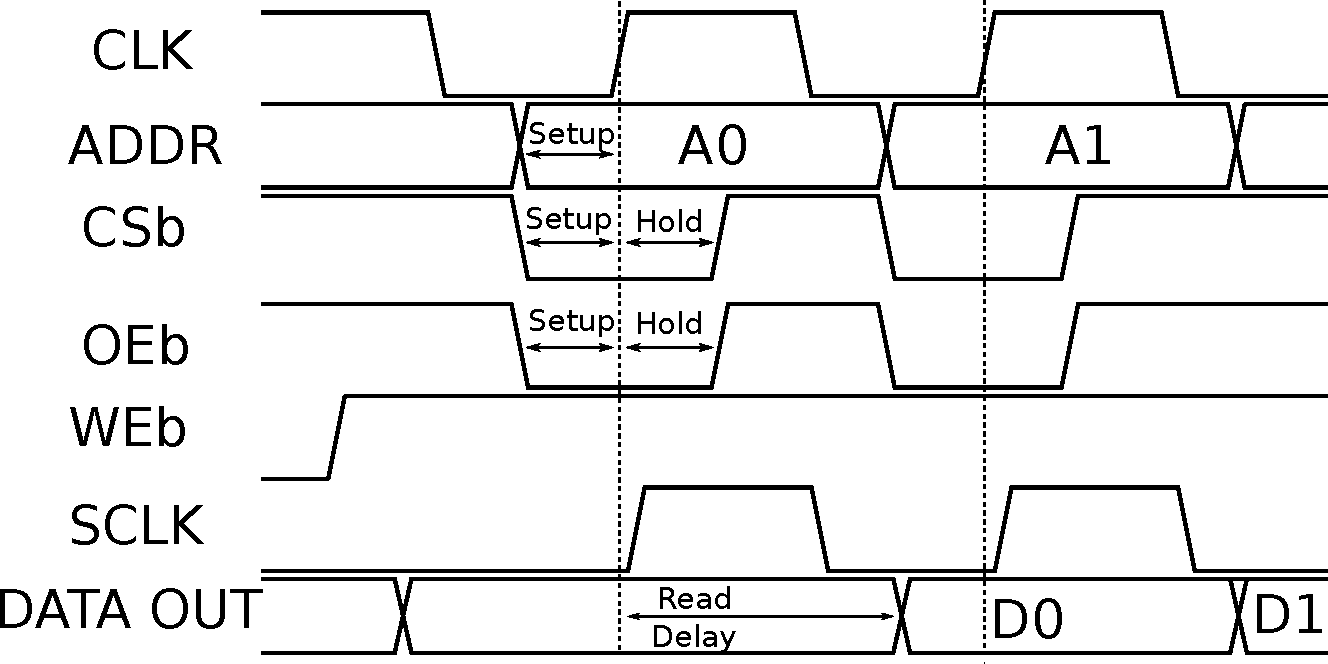
\includegraphics[width = 8cm]{figs/timing_read.pdf}
\label{fig:timing_read}}
\subfigure[Write operation timing]{
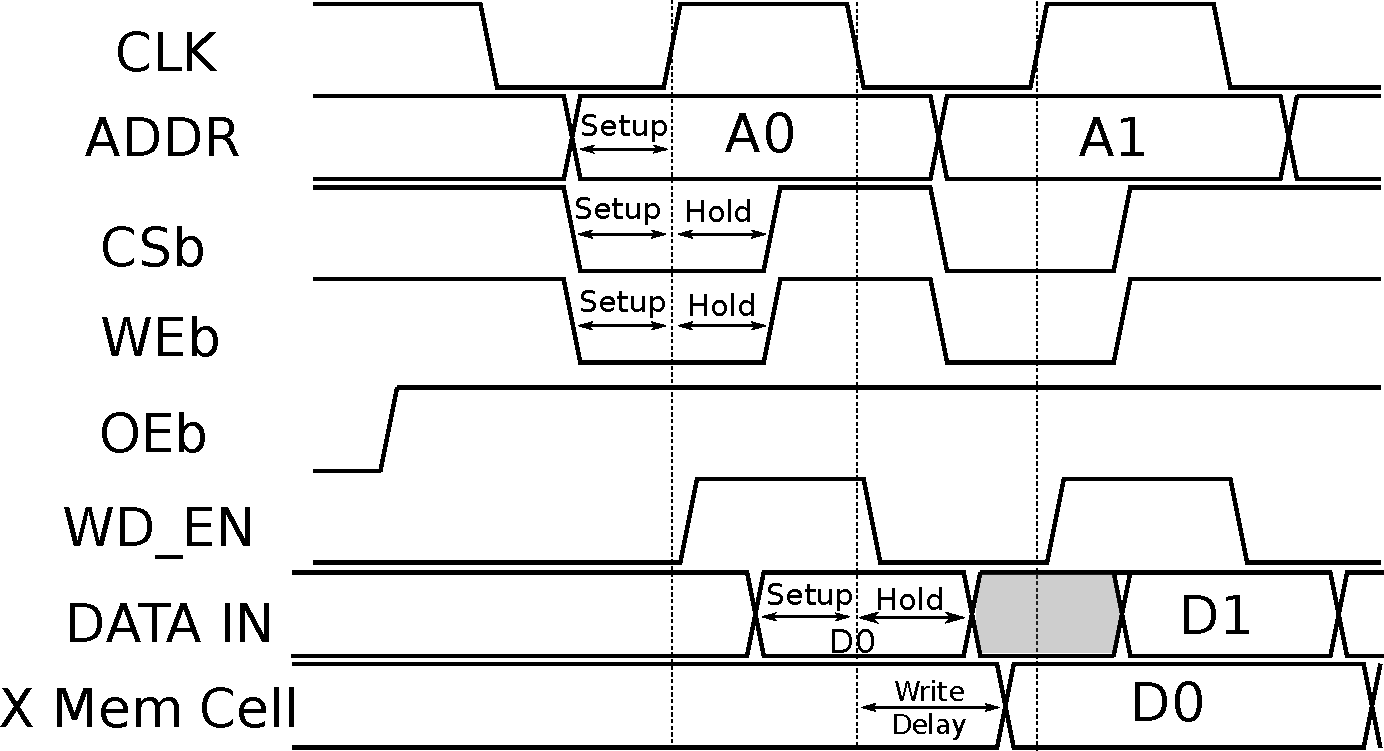
\includegraphics[width = 8cm]{figs/timing_write.pdf}
\label{fig:timing_write}}
\caption{OpenRAM uses a synchronous SRAM interface using a system
  clock (clk) along with control signals: output enable (OEb), chip
  select (CSb) and write enable (WEb).}
\label{fig:timing}
\end{figure*}

{\bf Bit-cell Array:} In the initial release of OpenRAM, the $6$T cell
is the default memory cell because it is the most commonly used cell
in SRAM devices. $6$T cells are tiled together with abutting word- and
bit-lines to make up the memory array.  The bit-cell array's aspect
ratio is made as square as possible using multiple columns of data
words. The memory cell is a custom designed library cell for each technology.
Other types of memory cells, such as $7$T, $8$T, and $10$T cells, can be used
as alternatives to the $6$T cell.

{\bf Address Decoder:} The address decoder takes the row address bits
as inputs and asserts the appropriate word-line so that the correct
memory cells can be read from or written to. The address decoder is
placed to the left of the memory array and spans the array's vertical
length. Different types of decoders can be used such as an included
dynamic NAND decoder, but OpenRAM's default option is a hierarchical CMOS
decoder.

{\bf Word-Line Driver:} Word-line drivers are inserted between the
address decoder and the memory array as buffers. The word-line drivers
are sized based on the width of the memory array so that they can drive
the row select signal across the bit-cell array.

{\bf Column Multiplexer:} The column multiplexer is an optional block
that uses the lower address bits to select the associated word in a
row. The column mux is dynamically generated and can be omitted or can
have 2 or 4 inputs. Larger column muxes are possible, but are not
frequently used in memories. There are options for a multi-level tree
mux as well.

{\bf Bit-line Precharge:} This circuitry pre-charges
the bit-lines during the first phase of the clock for read
operations. The precharge circuit is placed on top of every column in
the memory array and equalizes the bit-line voltages so that the
sense amplifier can sense the voltage difference between the two
bit-lines.

{\bf Sense Amplifier:} A differential sense amplifier is used to sense
the voltage difference between the bit-lines of a memory cell while a
read operation is performed.  The sense amplifier uses a bit-line
isolation technique to increase performance. The sense amplifier
circuitry is placed below the column multiplexer or the memory
array if no column multiplexer is used. There is one sense amplifier for
each output bit.

{\bf Write Driver:} The write drivers send the input data signals onto the
bit-lines for a write operation. The write drivers are tri-stated
so that they can be placed between the column multiplexer/memory array
and the sense amplifiers. There is one write driver for each input
data bit.

%% \subsubsection{Bit-cell and Bit-cell Array}
%% A bit-cell class is provided to instantiate the custom designed memory
%% cell located in the technology directory. Then the bit-cell array class
%% will take the single bit-cell instance to dynamically generate the
%% memory array. Using the functionality of GdsMill, we can rotate and/or
%% mirror an instance. Doing so, will allow us to abut the power rails.

%% \subsubsection{Address Decoder}
%% The hierarchical decoder is the default row address decoder that is
%% used in OpenRAM. The hierarchical decoder is dynamically generated
%% using the inverter and NAND gates with the help of basic shapes. The
%% height of each decoder row will match the height of the memory cell so
%% that the power rails can be abutted. OpenRAM also provides a NAND
%% decoder as an alternative. NAND decoder uses NMOS and PMOS transistors
%% created by ptx class. User can define type of the decoder in the
%% configuration file.

%% \subsubsection{Word-line Driver}
%% The word-line driver will be a column of alternating "mirrored"
%% inverters instances that is used to drive the signal to access the
%% memory cells in the row. The inverters will be sized accordingly
%% depending on the size of the memory array.

%% \subsubsection{Column Multiplexer}
%% The column multiplexer is an optional block that is used depending on
%% the size of the memory array. By generating an instance of a 1-1
%% multiplexer, we can then tile them to create bigger multiplexers such
%% as 2-1, 4-1, etc. OpenRAM has two options for column multiplexing.
%% Single-level-column-mux is the default column multiplexer but user can
%% choose Tree-Column-Mux in configuration file.  Both multiplexers use
%% transistors created by ptx class.

%% \subsubsection{Precharge and Precharge Array}
%% The precharge circuitry is dynamically generated using the transistor
%% instances and various basic shapes. The precharge class dynamically
%% generates an instance for a single column. The precharge array class
%% takes that instance and tiles them horizontally to match the number of
%% columns in the memory array. The width of the precharge cell is
%% determined by the width of the user-created memory cell.

%% \subsubsection{Sense Amplifier and Sense Amplifier Array}
%% The sense amplifier is user-designed analog circuit that is placed in
%% the technology directory. The sense amplifier class instantiates the
%% library cell and the sense amplifier array takes that instance to
%% create a horizontal array matching the number of output bits for the
%% memory. When designing this library cell, the user should match this
%% cell's width and bit-lines to the memory cell's.

%% \subsubsection{Write Driver and Write Driver Array}
%% Similar to the precharge classes, the write driver class will generate
%% an instance for a single bit and the write driver array will tile them
%% horizontally to match the number of input bits for the memory. The
%% write drivers will be dynamically sized accordingly based on the size
%% of the memory array.

%% \subsubsection{Control Logic}
%% There will be a control logic module that will arrange the
%% master-slave flip-flops and the logic associated with the control
%% signals into a single design. Flip-flops are used to drive the control
%% signals and standard library cells such as NAND and NOR gates will be
%% used for the logic.  A RBL is also generated using parameterized gates
%% and Replica Cell (RC). RC is a 6T SRAM memory cell which is hard-wired
%% to store a zero in order to discharge the RBL and generate the sense
%% amplifier enable signal in read mode.

%% \subsubsection{Additional Arrays}
%% In addition to the eight main blocks, there are helper modules that
%% help simplify the designs in the eight main blocks. We have a
%% flip-flop array class that takes the custom designed master-slave
%% flip-flop library cell to create a tiled array.  We also have the
%% tri-state array class that will generate the array of tri-states for
%% the DATA bus.

% Overview of signal inputs and timing
{\bf Control Logic:} The OpenRAM SRAM architecture incorporates a
standard synchronous memory interface using a system clock (clk). The
control logic uses an externally provided, active-low output enable
(OEb), chip select (CSb), and write enable (WEb) to combine multiple
SRAMs into a larger structure. Internally, the OpenRAM compiler can
have $1$, $2$, or $4$ memory banks to amortize the area/power cost of
control logic and peripheral circuitry.

All of the input control signals are stored using master-slave (MS)
flip-flops (FF) to ensure that the signals are valid for the entire
clock cycle. During a read operation, data is available after the
negative clock edge (second half of cycle) as shown in
Figure~\ref{fig:timing_read}. To avoid dead cycles which degrade
performance, a Zero Bus Turn-around (ZBT) technique is used in OpenRAM
timing. The ZBT enables higher memory throughput since there are no
wait states. During ZBT writes, data is set up before the negative
clock edge and is captured on the negative edge. Figure~\ref{fig:timing_write}
shows the timing for input signals during the write operation.

The internal control signals are generated using a replica bit-line (RBL)
structure for the timing of the sense amplifier enable and output
data storage~\cite{RBL:1998}. The RBL turns on the sense amplifiers 
at the exact time in presence of process variability in sub-$100$nm 
technologies.

